%%%%%%%%%%%%%%%%%%%%%%%%%%%%%%%%%%%%%%%%%%%%%%%%%%%%%%%%%%%%%%%%%%%%%%%%%%%
%
% Plantilla para un artículo en LaTeX en español.
%
%%%%%%%%%%%%%%%%%%%%%%%%%%%%%%%%%%%%%%%%%%%%%%%%%%%%%%%%%%%%%%%%%%%%%%%%%%%

% Qué tipo de documento estamos por comenzar:
\documentclass[a4paper]{article}
% Esto es para que el LaTeX sepa que el texto está en español:
\usepackage[spanish]{babel}
\selectlanguage{spanish}
% Esto es para poder escribir acentos directamente:
\usepackage[utf8]{inputenc}
\usepackage[T1]{fontenc}
\usepackage{float}

\usepackage{enumerate} 

%% Asigna un tamaño a la hoja y los márgenes
\usepackage[a4paper,top=3cm,bottom=2cm,left=3cm,right=3cm,marginparwidth=1.75cm]{geometry}

%% Paquetes de la AMS
\usepackage{amsmath, amsthm, amsfonts}
%% Para añadir archivos con extensión pdf, jpg, png or tif
\usepackage{graphicx}
\usepackage[colorinlistoftodos]{todonotes}
\usepackage[colorlinks=true, allcolors=blue]{hyperref}

%% Primero escribimos el título
\title{Analisis de algoritmos de ordenamiento }
\author{Bejar Merma Ángel Andrés\\
  \small Universidad Nacional de San Agustin\\
  \small andresbjar97@gmail.com\\
  \small Ciudad de Arequipa
  \date{}
}

%% Después del "preámbulo", podemos empezar el documento

\begin{document}
%% Hay que decirle que incluya el título en el documento
\maketitle

%% Aquí podemos añadir un resumen del trabajo (o del artículo en su caso) 
\begin{abstract}
El trabajo consiste en un análisis del rendimiento de un conjunto de algoritmos en función de su tiempo de ejecución con diferentes conjuntos de datos tanto para c++ como para Python.
Se  prueban, comparan y concluye qué algoritmo es mejor para conjuntos de datos pequeños, promedio, veremos el peor caso, caso promedio y mejor.

\end{abstract}

%% Iniciamos "secciones" que servirán como subtítulos
%% Nota que hay otra manera de añadir acentos
\section{Introducci\'on}

La ordenación es una de las cuestiones importantes  en computación  el problema de ordenación es importante porque de eso depende otros algoritmos los que los hacen mas o menos eficientes uno de de estos algoritmos es el algoritmo de búsqueda .

El concepto clave  es algoritmo ,un algoritmo se puede definir como una  secuencia de  pasos   bien definidos para resolver un problemas . El algoritmo toma una entrada y proporciona una salida.\cite{5376871}
Se han propuesto varios algoritmos de ordenación con diferentes restricciones, p. Ej. número de iteraciones (bucle interno, bucle externo), complejidad y problema de consumo de CPU.












\section{Marco Teórico}

Los algoritmos de ordenamiento se dividen en dos categorías bien diferenciadas:el Bubble Sort, Insertion Sort ,y Selection Sort en la categoría de O($n^{2}$), mientras que Quick Sort  y Merge Sort  
O(n log n).La descripción de cada uno de ellos a continuación.

\begin{enumerate}[a)]

\item \textbf{Bubble sort:}
El algoritmo de ordenacion básico es la clasificación de burbujas. Compara dos elementos adyacentes y realiza una operación de intercambio si se encuentra un pedido incorrecto con pasos repetidos. Esto también se denomina algoritmo de ordenación  por comparación.Una de sus ventajas es sus facil  implementacion 

\item \textbf{Heap sort:}
La ordenacion de montón es una técnica de clasificación basada en comparaciones basada en la estructura de datos binary heap. Es similar a ordenamiento por selección donde primero encontramos el elemento mínimo y colocamos el elemento mínimo al principio. Repetimos el mismo proceso para el resto de elementos\cite{heap}.

\item \textbf{Insertion sort}
\\
El ordenamiento por inserción (insertion sort en inglés) es una manera muy natural de ordenar para un ser humano, y puede usarse fácilmente para ordenar un mazo de cartas numeradas en forma arbitraria. Requiere O($n^{2}$) operaciones para ordenar una lista de  n elementos.

Inicialmente se tiene un solo elemento, que obviamente es un conjunto ordenado. Después, cuando hay  k elementos ordenados de menor a mayor, se toma el elemento k+1 y se compara con todos los elementos ya ordenados, deteniéndose cuando se encuentra un elemento menor (todos los elementos mayores han sido desplazados una posición a la derecha) o cuando ya no se encuentran elementos (todos los elementos fueron desplazados y este es el más pequeño). En este punto se inserta el elemento k + 1 debiendo desplazarse los demás elementos\cite{inser}.

\item \textbf{ Shell sort}

ShellSort es principalmente una variación de Insertion Sort. En la ordenación por inserción, movemos los elementos solo una posición adelante. Cuando un elemento debe moverse mucho más adelante, se involucran muchos movimientos. La idea de shellSort es permitir el intercambio de elementos lejanos. En shellSort, hacemos que la matriz esté ordenada por h para un valor grande de h. Seguimos reduciendo el valor de h hasta que se convierte en 1. Se dice que una matriz está ordenada por h si todas las sublistas de cada elemento h están ordenadas\cite{shell}.

\item \textbf{Merge sort}

Este es un algoritmo de divide y conquista, con la ventaja  de fusionar listas con nuevas listas ordenadas. La complejidad del peor caso de la ordenación por fusión es O (nlog n), ya que podría usarse para conjuntos de datos grandes y peores. 
La ordenación por fusión utiliza los siguientes tres pasos \cite{merge} 

\begin{enumerate}[1)]
\item \textbf{Divide:}Si el tamaño de la matriz es mayor que 1, divídalo en dos subarreglos iguales de la mitad del tamaño.
\item \textbf{Conquista:} ordenar ambas subarreglos por recursividad
\item \textbf{Fusiona:} Combine ambas arreglos ordenadas en uno de tamaño original. Esto le dará un arreglo ordenada completo.


\end{enumerate}



 La ordenación por fusión es más adecuada para casos grandes y peores, pero usa más memoria en comparación con otros algoritmos de división y conquista. El algoritmo de clasificación de fusión se describe a continuación

\item \textbf{Quick sort}


\end{enumerate}


3.1 Clasificación de burbujas: el algoritmo de clasificación básico es la clasificación de burbujas. Compara dos elementos adyacentes y realiza una operación de intercambio si se encuentra un pedido incorrecto con pasos repetidos. Esto también se denomina algoritmo de clasificación por comparación [7]. El tipo de burbuja original lo hace 


\section{Metodología}

Lo que se hizo fue probar los algoritmos de ordenamiento  en Python 
utilizando Google colab y el entorno de ejecución GPU. La maquina que nos asigno google fue una Tesla k80 se intento reiniciar el entono para obtener una tesla t 40 , pero fue inútil.

Para la pruebas en c++
La computadora  que utilizo es una intel i5 de quinta generación  con 2 cores ,8 gb  de memoria ram 

Los algoritmos escogidos son los siguientes:

\begin{itemize}


\item  Bubble sort

\item Heap sort

\item Insertion sort

\item Selection sort

\item Shell sort

\item  Merge sort

\item Quick sort

\end{itemize}

Como datos de entrada usaremos libreoffice para graficar los resultados.

Con  respecto a la ejecución de los algoritmos de python  en Google Colab el proceso tardo mas de 8 horas en terminar de ejecutarse se hizo la prueba en mi pc y tardo 1 hora  menos ,al ordenar 1000 000 elementos de un arreglo.

En el lenguaje de c se hizo una prueba con 100000 elementos 

En el lenguaje de c++ se hizo una prueba con 100000 elementos 

en c se hizo una prueba de 1000 001 de elementos 











\section{Resultados}


\begin{figure}[H]%primero aqui sino arriba sino abajo
\centering
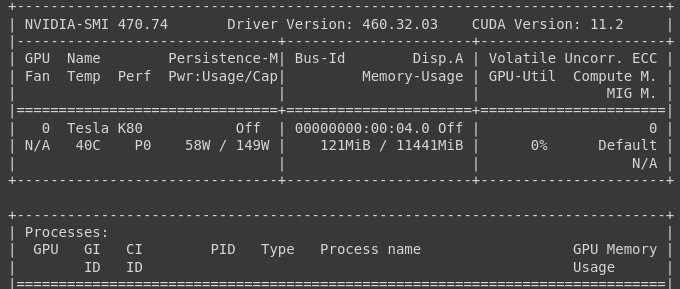
\includegraphics[width=10cm]{imagenes/arq2.png}
\caption{Gpu TeslaK80}
\end{figure}

\begin{figure}[H]%primero aqui sino arriba sino abajo
\centering
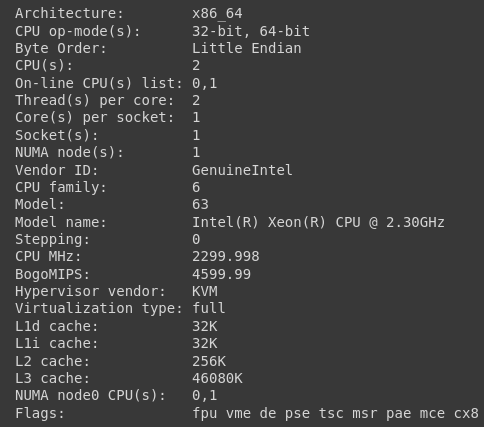
\includegraphics[width=7cm]{imagenes/arquitectura2.png}
\caption{Especificaciones Entorno Colab}
\end{figure}


\begin{figure}[H]%primero aqui sino arriba sino abajo
\centering
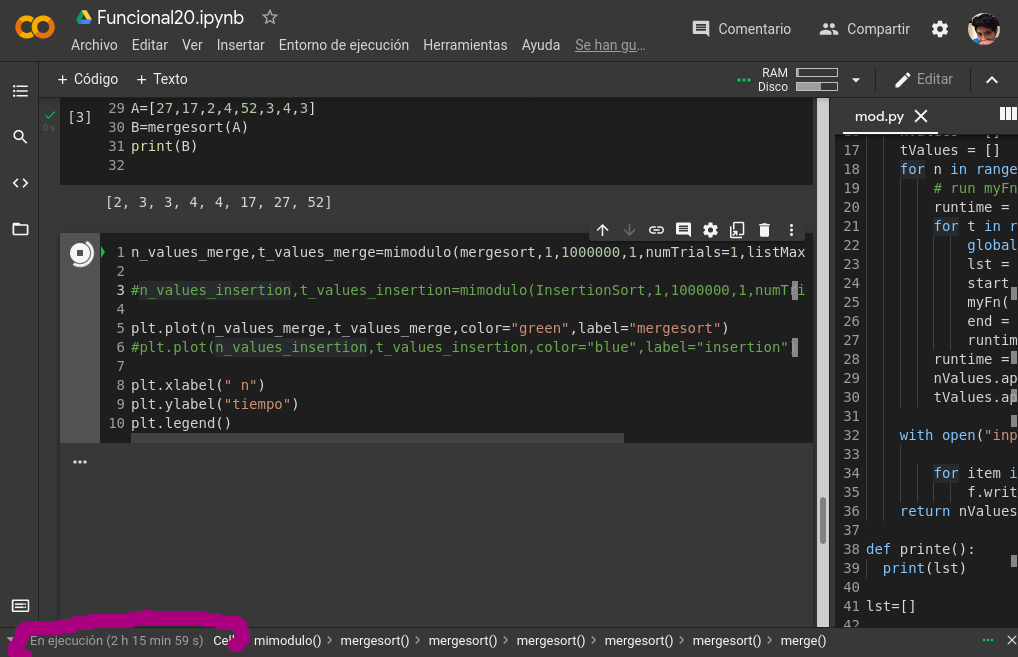
\includegraphics[width=14cm]{imagenes/cap.png}
\caption{Momento ejecutar codigo en python }
\end{figure}

\begin{figure}[H]%primero aqui sino arriba sino abajo
\centering
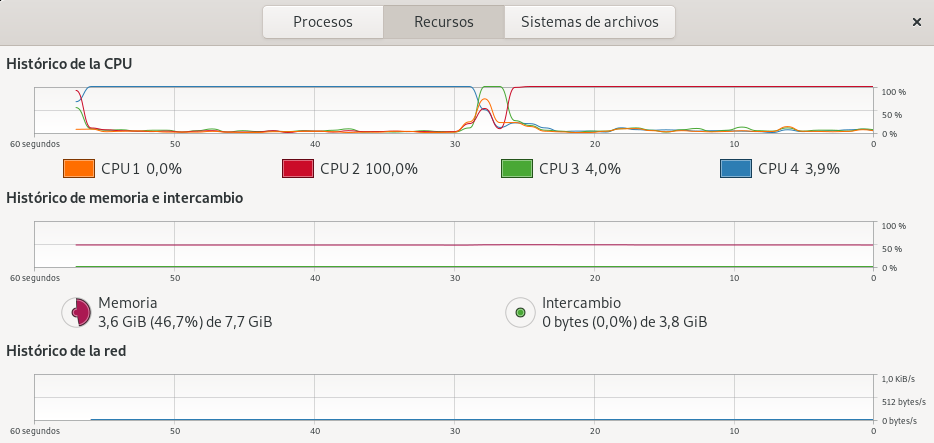
\includegraphics[width=13cm]{imagenes/cpus.png}
\caption{Uso de una core al 100 por ciento}
\end{figure}


cuaderno de trabajo
\cite{colab}


\begin{figure}[H]%primero aqui sino arriba sino abajo

\centering
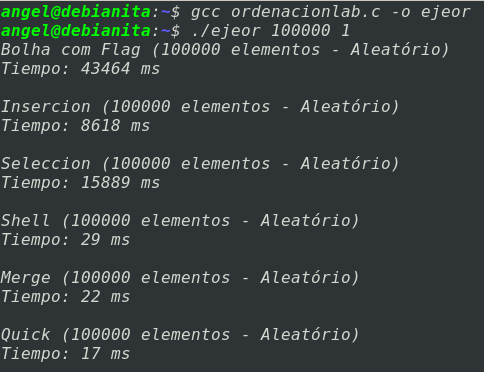
\includegraphics[width=10cm]{imagenes/t100milc.png}
\caption{Ejecutado en c con 100 mil elementos aleatorios}

\end{figure}

\begin{figure}[H]%primero aqui sino arriba sino abajo

\centering
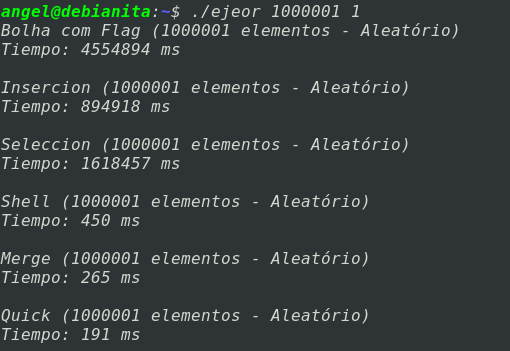
\includegraphics[width=10cm]{imagenes/millon.png}
\caption{Con 1 millon de elementos}

\end{figure}
\section{Conclusiones}


Es importante establecer el paralelismo entre el ordenamiento por selección y el ordenamiento por inserción. La selección realiza menos cambios (intercalación) que la inserción, ya que solo hay un cambio por iteración, es decir, en el orden de selección total hace n
intercambios. La ordenación por inserción, por otro lado, realiza al menos un cambio por iteración, ya que debe realizar cambios para eliminar cada elemento evaluado.

La ordenación por inserción, por otro lado, realiza menos comparaciones que la ordenación por selección, ya que el elemento que se va a insertar de forma ordenada no siempre tiene que llegar hasta el final. De hecho, esto solo ocurre en el peor de los casos, donde la matriz se ordena en orden inverso. La clasificación por selección necesita comparar todos los elementos restantes cada vez para determinar quién es el más pequeño.

En teoría, ambos pertenecen a la misma clase de complejidad, a saber, O ($n^{2}$)

. En la práctica, la ordenación por inserción funciona mejor que la ordenación por selección.

Finalmente, la clasificación por selección no se considera un algoritmo eficiente para entradas grandes. Hay alternativas O (nlogn)
, como Quick Sort y Merge Sort, así como alternativas lineales como Counting Sort. 


La ordenación por fusión o Merge Sort es más adecuada para casos grandes y peores, pero usa más memoria en comparación con otros algoritmos de división y conquista.

\cite{rin}

La complejidad de Quick Sort en los casos mejores y medios  es O(nlogn) y en el peor de los casos O( $n^{2}$)  . La complejidad media del tiempo de caso es O(nlogn) que es un poco costosa si se utiliza para grandes conjuntos de datos, también en el peor de los casos la complejidad es O($n^{2}$), lo que lo hace impráctico para los peores conjuntos de datos grandes.

\section{Discusión}




\bibliographystyle{plain}
\bibliography{referencias}




\end{document}
